\documentclass{article}
\usepackage{amsmath, amssymb, amsthm, enumerate, graphicx}
\usepackage[usenames,dvipsnames]{color}
\usepackage{bm}
\usepackage[colorlinks=true,urlcolor=blue]{hyperref}
\usepackage{geometry}
\geometry{margin=1in}
\usepackage{float}
\usepackage{graphics}
\setlength{\marginparwidth}{2.15cm}
\usepackage{booktabs}
\usepackage{enumitem}
\usepackage{epsfig}
\usepackage{setspace}
\usepackage{parskip}
\usepackage{enumerate}
\usepackage[normalem]{ulem}
\usepackage{tikz}
\usetikzlibrary{positioning, arrows, automata}
\usepackage{pgfplots}
\usepackage[font=scriptsize]{subcaption}
\usepackage{float}
\usepackage[]{algorithm2e}
\usepackage{environ}
\usepackage{bbm}
\usepackage{graphicx}
\usepackage{titling}
\usepackage{url}
\usepackage{color}
\usepackage{xcolor}
\usepackage{lipsum}
\usepackage{lastpage}
\usepackage[colorlinks=true,urlcolor=blue]{hyperref}
\usepackage{multicol}
\usepackage{tabularx}
\usepackage{comment}
\usepackage[utf8]{inputenc}
\usepackage{amssymb}
\usepackage{setspace}
\usepackage{marvosym}
\usepackage{wrapfig}
\usepackage{datetime}
\usepackage[many]{tcolorbox}
\usepackage{array}
\usepackage{multirow}
\usepackage{wasysym}
\usepackage{cancel}
\usepackage{framed}

\usepackage{listings}
\usepackage{color}

\newcommand{\R}{\mathbb{R}}
\newcommand{\blackcircle}{\tikz\draw[black,fill=black] (0,0) circle (1ex);}
\renewcommand{\circle}{\tikz\draw[black] (0,0) circle (1ex);}
\newcommand{\eMLE}{\widehat{\theta}_{\text{MLE}}}


\newtcolorbox[]{your_solution}[1][]{
    % breakable,
    enhanced,
    nobeforeafter,
    colback=white,
    title=Your Answer,
    sidebyside align=top,
    box align=top,
    #1
}

% Custom functions
\newcommand{\vind}[1]{\mathbbm{1}_{#1}}
\newcommand{\Lagr}{\mathcal{L}}


% SOLUTION environment
\NewEnviron{soln}{
\leavevmode\color{red}\ignorespaces \textbf{Solution} \BODY }{}

% QUESTION AUTHORS environment
\NewEnviron{qauthor}{
\leavevmode\color{blue}\ignorespaces \textbf{Author} \BODY}{}

% TO ONLY SHOW HOMEWORK QUESTIONS, include following (else comment out):
%\RenewEnviron{soln}{}
%\RenewEnviron{qauthor}{}


% \newcommand{\norm}[1]{\lVert #1 \rVert}
% \newcommand{\st}{\mathrm{s.t.}}

\makeatletter
\newcommand{\removelatexerror}{\let\@latex@error\@gobble}
\makeatother

\newcommand{\argmax}{\mathop{\mathrm{argmax}}}
\newcommand{\argmin}{\mathop{\mathrm{argmin}}}

\pgfplotsset{compat=1.17}

%%%%%%%%%%%%%%%%%%%%%%%%%%%%%%%%%%%%%%%%%%%
% Code highlighting with listings         %
%%%%%%%%%%%%%%%%%%%%%%%%%%%%%%%%%%%%%%%%%%%

\definecolor{bluekeywords}{rgb}{0.13,0.13,1}
\definecolor{greencomments}{rgb}{0,0.5,0}
\definecolor{redstrings}{rgb}{0.9,0,0}
\definecolor{light-gray}{gray}{0.95}

\newcommand{\MYhref}[3][blue]{\href{#2}{\color{#1}{#3}}}%

\definecolor{dkgreen}{rgb}{0,0.6,0}
\definecolor{gray}{rgb}{0.5,0.5,0.5}
\definecolor{mauve}{rgb}{0.58,0,0.82}

\lstdefinelanguage{Shell}{
  keywords={tar, cd, make},
  %keywordstyle=\color{bluekeywords}\bfseries,
  alsoletter={+},
  ndkeywords={python, py, javac, java, gcc, c, g++, cpp, .txt, octave, m, .tar},
  %ndkeywordstyle=\color{bluekeywords}\bfseries,
  identifierstyle=\color{black},
  sensitive=false,
  comment=[l]{//},
  morecomment=[s]{/*}{*/},
  commentstyle=\color{purple}\ttfamily,
  stringstyle=\color{red}\ttfamily,
  morestring=[b]',
  morestring=[b]",
  backgroundcolor = \color{light-gray}
}

\lstset{columns=fixed, basicstyle=\ttfamily,
    backgroundcolor=\color{light-gray},xleftmargin=0.5cm,frame=tlbr,framesep=4pt,framerule=0pt,
    showstringspaces=false}

%%%%%%%%%%%%%%%%%%%%%%%%%%%%%%%%%%%%%%%%%%%
% Custom box for highlights               %
%%%%%%%%%%%%%%%%%%%%%%%%%%%%%%%%%%%%%%%%%%%

% Define box and box title style
\tikzstyle{mybox} = [fill=blue!10, very thick,
    rectangle, rounded corners, inner sep=1em, inner ysep=1em]

% \newcommand{\notebox}[1]{
% \begin{tikzpicture}
% \node [mybox] (box){%
%     \begin{minipage}{\textwidth}
%     #1
%     \end{minipage}
% };
% \end{tikzpicture}%
% }

\NewEnviron{notebox}{

\begin{tikzpicture}
\node [mybox] (box){
    \begin{minipage}{\textwidth}
        \BODY
    \end{minipage}
};
\end{tikzpicture}
}

\begin{document}
\section*{}
\begin{center}
  \centerline{\textsc{\LARGE  Homework 1}}
  \vspace{0.5em}
  \centerline{\textsc{\LARGE Decision Trees and kNN}
  %\footnote{Compiled on \today{} at \currenttime{}}
  }
  \vspace{1em}
  \textsc{\large UTK COSC 522: Machine Learning (Fall 2025)} \\
  \vspace{0.5em}
  %\url{piazza.com/cmu/spring2024/10701/home} \\
  %\vspace{0.5em}
  \centerline{OUT: Tuesday, Sep 2nd, 2025}
  %\today{} at \currenttime{}}}
  \vspace{0.5em}
  \centerline{DUE: Wednesday, Sep 17th, 2025, 11:59pm EST}
\end{center}

\section*{Homework Instructions}
\begin{itemize}
\item \textbf{Collaboration policy: Taking Responsibility for Your Career} 

The skills you learn in this course are tools for your future, and this policy is designed to help you sharpen them. You are responsible for your own learning and career, and this framework ensures you get the most from every assignment.

We encourage collaboration, but it must be done \emph{right}. \emph{First}, make a genuine effort to solve problems on your own. This independent effort is where the most critical learning occurs. \emph{Afterward}, you may discuss strategies with peers or consult resources to clarify concepts—the goal is to deepen your own understanding, not to simply get an answer.

\emph{Finally}, like any professional, you must stand behind your own work. Your submitted solution must be written entirely by you, from scratch, without collaborators present. This proves you have truly mastered the material. To maintain academic and professional integrity, you must also cite any person or resource that contributed to your understanding along the way. 

\item\textbf{Late Submission Policy:} See the late homework policy here: \url{https://docs.google.com/document/d/1lYopNzjn_0AOipRiiwO4h2Ow64seQNeD/edit?usp=sharing&ouid=114000599194691965836&rtpof=true&sd=true}

\item\textbf{Submitting your work:} 

\begin{itemize}

\item \textbf{Canvas:} 
For this homework, you will submit a \textbf{single .zip file} to Canvas. Please name your file in the format \textbf{YourName\_NetID\_HW1.zip}. This zip file must contain exactly two files: your written solutions in a single PDF and your Python code.

Your \textbf{single PDF file} must contain your answers to all questions, including written problems (proofs, short answers, plots) and the empirical questions from the programming section. You must use the provided homework template. Using the LaTeX version to typeset is strongly recommended, but you may also submit a scan of the template with legible handwriting; \textbf{illegible answers will not be graded}. Please complete all answers within the provided boxes. 

The second file in your zip archive must be your \emph{single} completed programming file, named exactly as \textbf{decision\_tree.py}. Please ensure your code is runnable, as we may execute it to verify your results.

Regrade requests can be made after homework grades are released. Please be aware that a regrade request allows the TA to review your entire assignment, which may result in points being deducted if new errors are found.

\end{itemize}

\end{itemize}

For multiple-choice and select-all-that-apply questions, please shade the corresponding box or circle to indicate your answer(s). If you are using the LaTeX template, use the $\blacksquare$ command for shaded boxes and $\blackcircle$ for shaded circles. \textbf{Note}: Do not alter the template in any other way. If a question includes a box for showing your work, you must \textbf{show your work} to receive full credit.



\clearpage


% added course policy section
% currently it is stated that these questions will not be graded, but must be finished

\section{Decision Trees [20 pts]}
\begin{enumerate}


\item Consider the dataset in Table \ref{dec_tab} for this problem. Given the four attributes on the left, we want to predict if the student got an A in the course. The following questions involve some computation, so you may want to solve them programmatically. You can find this dataset in \textit{data.txt}

\begin{table}[ht]
\begin{center}
\begin{tabular}{| c | c | c | c || c |} 
\hline
\vtop{\hbox{\strut \textbf{Wakes Up}}\hbox{\strut \textbf{Early}}} & \vtop{\hbox{\strut \textbf{Finished All}}\hbox{\strut \textbf{Homework}}} & \vtop{\hbox{\strut \textbf{Completed}}\hbox{\strut \textbf{Pre-requisites}}} & \textbf{Likes Coffee} & \textbf{A} \\ 
\hline
1 & 1 & 0 & 0 & 0\\ 
\hline
1 & 1 & 1 & 0 & 1\\ 
\hline
0 & 0 & 1 & 0 & 0\\ 
\hline
0 & 1 & 1 & 0 & 1\\ 
\hline
0 & 1 & 1 & 0 & 1\\ 
\hline
0 & 0 & 1 & 1 & 0\\ 
\hline
1 & 0 & 0 & 0 & 0\\ 
\hline
0 & 1 & 0 & 1 & 1\\ 
\hline
0 & 0 & 1 & 0 & 1\\ 
\hline
1 & 0 & 0 & 0 & 0\\ 
\hline
1 & 1 & 1 & 0 & 1\\ 
\hline
0 & 1 & 1 & 1 & 0\\ 
\hline
0 & 0 & 0 & 0 & 0\\ 
\hline
1 & 0 & 0 & 1 & 0\\ 
\hline
\end{tabular}
\end{center}
\caption{decision tree features and labels}
\label{dec_tab}
\end{table}

Create a decision tree of depth 2 using the ID3 algorithm from class. The tree should have the same structure as the diagram in Figure~\ref{fig:tree}. Note that 0 leads to the left branch and 1 leads to the right branch. 
\begin{figure}[ht]
\begin{center}
  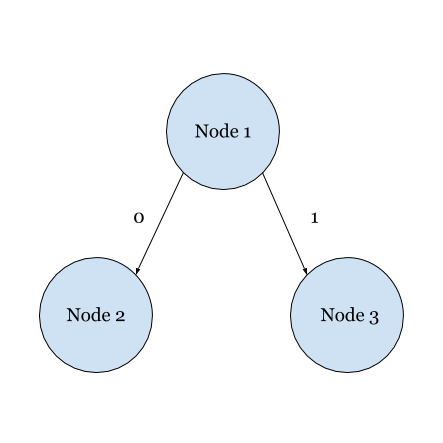
\includegraphics[width=5cm]{images/decisiontree.png}
\end{center}
  \caption{Decision tree structure for question 1}
\label{fig:tree}
\end{figure}
\begin{enumerate}[label=(\roman*)]

\newpage

\item \textbf{[4 pts]} What is the attribute at Node 1? What is the information gain of this attribute? Please round your answer to 4 decimal places.

Attribute to split on: \begin{tcolorbox}[fit,height=1.2cm, width=3.5cm, blank, borderline={1pt}{-2pt}, nobeforeafter, box align = center] \end{tcolorbox}
\hspace{0.5cm} Mutual information: \begin{tcolorbox}[fit,height=1.2cm, width=3.5cm, blank, borderline={1pt}{-2pt}, nobeforeafter, box align = center] \end{tcolorbox} 
 
    
\item \textbf{[4 pts]} What is the attribute at Node 2? What is the information gain of this attribute? Please round your answer to 4 decimal places.

Attribute to split on: \begin{tcolorbox}[fit,height=1.2cm, width=3.5cm, blank, borderline={1pt}{-2pt}, nobeforeafter, box align = center] \end{tcolorbox}
\hspace{0.5cm} Mutual information: \begin{tcolorbox}[fit,height=1.2cm, width=3.5cm, blank, borderline={1pt}{-2pt}, nobeforeafter, box align = center] \end{tcolorbox} 


\item \textbf{[4 pts]} What is the attribute at Node 3? What is the information gain of this attribute? Please round your answer to 4 decimal places. \\
\\
Note: If there is a tie on the attribute with the highest information gain, write any of the attribute that has the highest information gain.

Attribute to split on: \begin{tcolorbox}[fit,height=1.2cm, width=3.5cm, blank, borderline={1pt}{-2pt}, nobeforeafter, box align = center] \end{tcolorbox}
\hspace{0.5cm} Mutual information: \begin{tcolorbox}[fit,height=1.2cm, width=3.5cm, blank, borderline={1pt}{-2pt}, nobeforeafter, box align = center] \end{tcolorbox} 

    
\end{enumerate}

\item \textbf{[4 pts]} Consider learning a decision tree for some binary classification task. Assume that we do not restrict the size of the tree and that the tree can branch multiple times on the same attribute. Under what condition(s) would we be unable to construct a tree that perfectly classifies the dataset?  
\begin{tcolorbox}[fit,height=5cm, width=15cm, blank, borderline={1pt}{-2pt}]

\end{tcolorbox}


\item \textbf{[4 pts]} Given enough time, is the ID3 algorithm guaranteed to output the smallest decision tree that is \emph{consistent} with the training dataset i.e., achieves zero training error rate? Briefly explain why or why not. 
\begin{tcolorbox}[fit,height=5cm, width=15cm, blank, borderline={1pt}{-2pt}]
%solution
\end{tcolorbox}


\end{enumerate}
\newpage

\section{Nearest Neighbors and Decision Trees [6 Points]}

Consider a multiclass classification problem with 2 real-valued features. Suppose you are given $n$ data points $P_1, P_2, \ldots, P_n$ and the corresponding label for each data point $C_1, C_2, \ldots, C_n$ (where $C_1, C_2, \ldots, C_n$ take values from the set of all possible class labels). Under the $k$ nearest neighbors classification scheme, each new element $Q$ is simply categorized by a majority vote among its $k$ nearest neighbors. The 1-NN is a simple variant of this which divides up the input space for classification purposes into convex regions (see Figure \ref{fig:KNN_and_DT}), each corresponding to a point in the dataset.

\begin{figure}[H]
    \centering
    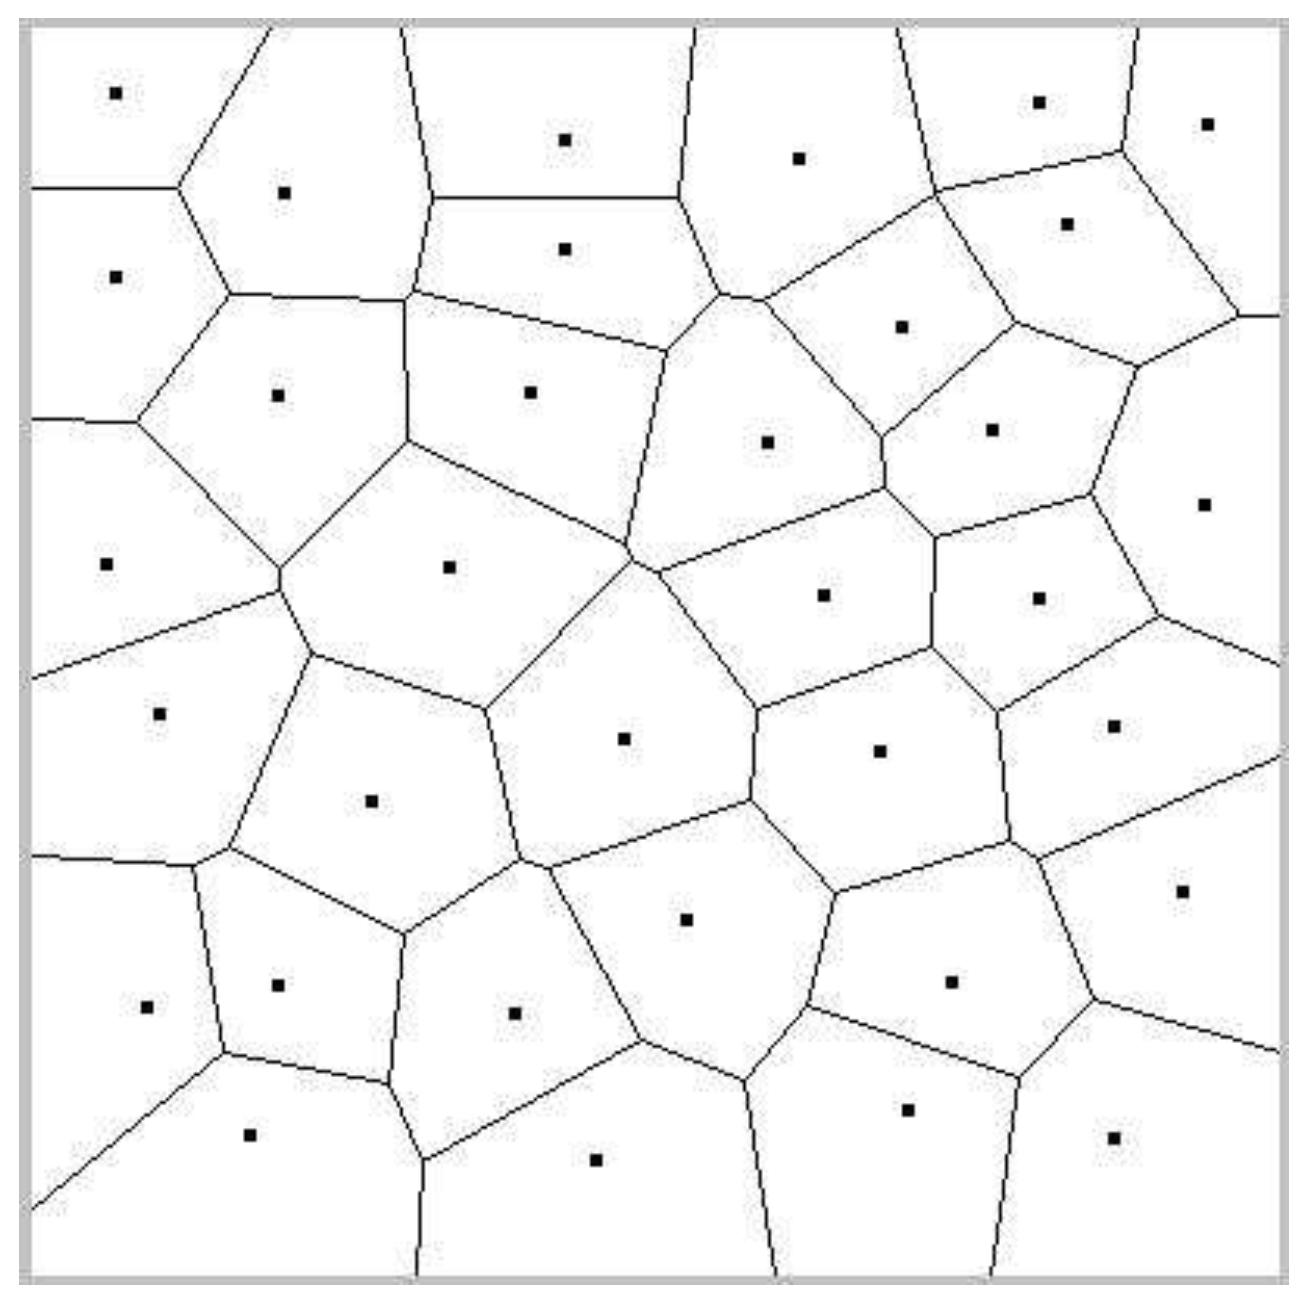
\includegraphics[width=0.5\textwidth]{images/1_KNN_and_DT.png}
    \caption{1-NN decision boundaries using the Euclidean distance metric.}
    \label{fig:KNN_and_DT}
\end{figure}
\begin{enumerate}

\item {\bf [6 Points]} Is it possible to build a decision tree (with decisions at each node of the form ``is $x_1 > a$'', ``is $x_1 < b$'', ``is $x_2 > c$'', or ``is $x_2 < d$'' for any real constants $a,b,c,d$) which behaves identically to a 1-NN classifier using the Euclidean distance metric? If so, how and if not, why not.

\begin{tcolorbox}[fit,height=7cm, width=15cm, blank, borderline={1pt}{-2pt}]

\end{tcolorbox}

\end{enumerate}
\newpage
\clearpage
\section{$k$-Nearest Neighbors [19 Points]}

\begin{enumerate}

        \item \textbf{[6 pts]} In a $k$NN classification problem, assume that the distance measure is not explicitly specified to you. Instead, you are given a “black box” where you input a set of data points $P_1, P_2, \dots P_n$ and an unlabelled data point $Q$, and the black box outputs the nearest neighbor of $Q$, say $P_i$ and its corresponding label $C_i$. Is it possible to construct a $k$NN classification algorithm (w.r.t the unknown distance metrics) based on this black box alone? If so, how and if not, why not?
        \begin{tcolorbox}[fit,height=7cm, width=0.9\textwidth, blank, borderline={1pt}{-2pt}]
        %solution 
        \end{tcolorbox}
        
        \item \textbf{[4 pts]} Now suppose the black box returns the $j$ nearest neighbors (and their corresponding labels) instead of the single nearest neighbor (assume $j \neq k$). Is it still possible to construct a $k$NN classification algorithm based on the black box? If so, how and if not, why not? You should separately discuss two scenarios: (1) the returned $k$-nearest neighbors are \emph{ordered/unoredered} based on the unknown distance metrics.  

        \textbf{Note:} The black box operates with a \emph{set} of data points, which assumes they are distinct.
        \begin{tcolorbox}[fit,height=7cm, width=0.9\textwidth, blank, borderline={1pt}{-2pt}]
        %solution 
        \end{tcolorbox}
        
\newpage
        \item \textbf{[3 pts]} Assume we have a dataset with binary labels and we know that the leave-one-out cross validation accuracy (LOOCV) of a $1$-NN classifier on this dataset is $1$. Now suppose that we introduce some noise to the dataset: each label has a 10\% chance of being flipped to the other class. What is the \emph{expected} LOOCV accuracy of a $1$-NN classifier in this setting? Note that the validation accuracy is always calculated with respect to the given ground-truth label, whether it being flipped or not. 
        

        \begin{tcolorbox}[fit,height=5cm, width=0.9\textwidth, blank,       borderline={1pt}{-2pt}]
        %solution 
        \end{tcolorbox}


        \item \textbf{[3 pts]} Suppose that in the dataset from the previous question, exactly $10 \%$ of the labels got flipped. What is the \emph{maximum} possible LOOCV accuracy (you can assume any data distribution in your preference)? Justify your answer using a formal proof or by constructing an example. 

        \begin{tcolorbox}[fit,height=3cm, width=0.9\textwidth, blank,       borderline={1pt}{-2pt}]
        %solution 
        \end{tcolorbox}

    
        \item \textbf{[3 pts]} How should the noise level (i.e., the probability of a label being flipped) affect your choice of $k$ for the $k$-NN algorithm, if at all? You do not need to provide a formal proof but you should give a brief justification. \emph{Hint:} think about variance-bias tradeoff in overfitting and underfitting scenarios.  

        \begin{tcolorbox}[fit,height=3cm, width=0.9\textwidth, blank,       borderline={1pt}{-2pt}]
        %solution 
        \end{tcolorbox}


    \clearpage
\end{enumerate}
\clearpage
\section{Programming (55 points)}

In this assignment, you will implement a decision tree learning algorithm for binary classification. In addition, we will ask you to run some end-to-end experiments on two tasks (predicting whether or not a patient has heart disease / predicting the final grade for high school students) and report your results. Please confine all code you write to a single, self-contained file titled \texttt{decision\_tree.py}. 


\subsection{The Tasks and Datasets}
\label{sec:data}

\paragraph{Materials} Download the zip file from the course website. The zip file will have a handout folder that contains all the data that you will need in order to complete this assignment.


\paragraph{Datasets}

The handout contains three datasets. Each one contains attributes and labels and is already split into training and validation data. The first line of each \lstinline{.tsv} file contains the name of each attribute, and \emph{the class label is always the last column}.

\begin{enumerate}
\item \textbf{heart:}
    The first task is to predict whether a patient has been (or will be) diagnosed with heart disease, based on available patient information. The attributes (aka. features) are: 
    \begin{enumerate}
        \item \lstinline{sex}: The sex of the patient---1 if the patient is male, and 0 if the patient is female.
        \item \lstinline{chest_pain}: 1 if the patient has chest pain, and 0 otherwise.
        \item \lstinline{high_blood_sugar}: 1 if the patient has high blood sugar ($>$120 mg/dl fasting), and 0 otherwise.
        \item \lstinline{abnormal_ecg}: 1 if the patient had an abnormal resting electrocardiographic (ECG) reading, and 0 otherwise. 
        \item \lstinline{angina}: 1 if exercise induced angina in the patient, and 0 otherwise. Angina is a type of severe chest pain.
        \item \lstinline{flat_ST}: 1 if the patient's ST segment (a section of an ECG) was flat during exercise, and 0 if it had some slope.
        \item \lstinline{fluoroscopy}: 1 if a physician used fluoroscopy, and 0 otherwise. Fluoroscopy is an imaging technique used to see the flow of blood through the heart.
        \item \lstinline{thalassemia}: 1 if the patient is known to have thalassemia, and 0 otherwise. Thalassemia is a blood disorder that may impair the oxygen-carrying capacity of the patient's red blood cells.
        \item \lstinline{heart_disease}: 1 if the patient was diagnosed with heart disease, and 0 otherwise. This is the class label you should predict.
    \end{enumerate}
    The training data is in \lstinline{heart_train.tsv}, and the validation data in \lstinline{heart_valid.tsv}.
\item \textbf{education:}
    The second task is to predict the final grade for high school students. The attributes are student grades on 5 multiple choice assignments \emph{M1} through \emph{M5}, 4 programming assignments \emph{P1} through \emph{P4}, and the final exam \emph{F}. Values of 1 indicate that a student received an A, and 0 indicates that the student did not receive an A. The training data is in \newline \lstinline{education_train.tsv}, and the validation data in \lstinline{education_valid.tsv}.
\item \textbf{small:}
    We also include \lstinline{small_train.tsv} and \lstinline{small_valid.tsv}---a small, purely for demonstration version of the \textbf{heart} dataset, with \emph{only} attributes \lstinline{chest_pain} and \lstinline{thalassemia}.  

\end{enumerate}



\newpage
\subsection{Program: Decision Tree}
\label{sec:decisiontree}

Your code should learn a decision tree with a specified maximum depth, print the decision tree in a specified format, predict the labels of the training and validation examples, and calculate training and validation errors.


\textbf{Your implementation must satisfy the following requirements:}
\begin{itemize}
\item Use mutual information to determine which attribute to split on.
\item Be sure you’re correctly weighting your calculation of mutual information. For a split on attribute X, $I(Y;X) = H(Y)-H(Y|X) = H(Y) - P(X=0)H(Y|X = 0) - P(X = 1)H(Y|X = 1)$.
\item As a stopping rule, only split on an attribute if the mutual information is $>$ certain threshold. By default, you should set the threshold to $0$. Certain questions in \ref{sec:empirical questions} may require you to experiment with different threshold.
\item Do not grow the tree beyond a certain max-depth, if specified in the question. For example, for a maximum depth of 3, split a node only if the mutual information is $>$ 0 and the current level of the node is $< 3$.
\item Use a majority vote of the labels at each leaf to make classification decisions. If the vote is tied, choose the label that is numerically larger (i.e., $1$ should be chosen before $0$)
\item It is possible for different columns to have equal values for mutual information. In this case, you should split on the \emph{\textbf{first column to break ties}} (e.g. if column 0 and column 4 have the same mutual information, use column 0).
\end{itemize}

\subsubsection{Getting Started}
\label{sec:getting started}

Careful planning will help you to correctly and concisely implement your decision tree learning algorithm. Here are a few \emph{hints} to get you started:
\begin{itemize}
    \item Write helper functions to calculate entropy and mutual information.
    \item It is best to think of a decision tree as a collection of nodes, where nodes are either leaf nodes (where final decisions are made) or interior nodes (where we split on attributes). It is helpful to design a function to train a single node (i.e. a depth-0 tree), and then recursively call that function to create sub-trees.
    \item In the recursion, keep track of the depth of the current tree so you can stop growing the tree beyond the max-depth.
    \item Implement a function that takes a learned decision tree and data as inputs, and generates predicted labels. You can write a separate function to calculate the error of the predicted labels with respect to the given (ground-truth) labels.
    \item Be sure to correctly handle the case where the specified maximum depth is greater than the total number of attributes.
    \item Be sure to handle the case where max-depth is zero (i.e. a majority vote classifier). 

\end{itemize}


\clearpage

\subsubsection{Output: Printing the Tree}
\label{sec:printtree}

You should also write a function to pretty-print your learned decision tree. \textbf{Your function should print your tree only \emph{after} you are done generating the fully-trained tree.} Each row should correspond to a node in the tree. They should be printed using a \emph{pre-order depth-first-search} traversal (but you may print left-to-right or right-to-left, i.e. your answer does not need to have exactly the same order as the reference below). Print the \texttt{attribute} of the node's parent (e.g., \texttt{chest\_-pain} in example format below) and the \texttt{attribute value} corresponding to the node (e.g., value of 0 for \texttt{chest\_-pain}). Also include the sufficient statistics (i.e. count of negative (label as 0) / positive examples (label as 1)) for the data passed to that node. The row for the root should include \emph{only} those sufficient statistics. A node at depth $d$, should be prefixed by $d$ copies of the string `$\mid$ '.

Below, we have provided the recommended format for printing the tree (the \texttt{2} in the python command below denotes the maximum tree depth). You can print it directly rather than to a file. 

\begin{lstlisting}[language=Shell]
$ python decision_tree.py small_train.tsv small_valid.tsv 2

[14 0/14 1]
| chest_pain = 0: [4 0/12 1]
| | thalassemia = 0: [3 0/4 1]
| | thalassemia = 1: [1 0/8 1]
| chest_pain = 1: [10 0/2 1]
| | thalassemia = 0: [7 0/0 1]
| | thalassemia = 1: [3 0/2 1]
\end{lstlisting}


However, you should be careful that the tree might not be full. For example, with a different subset of the small dataset, there may be no nodes under \lstinline{chest_pain = 0} if all labels are the same.

The following pretty-print shows the education dataset with max-depth 3.  Use this example to check your code before submitting your pretty-print of the heart dataset.

\begin{lstlisting}[language=Shell]
$ python decision_tree.py education_train.tsv education_valid.tsv 3

[65 0/135 1]
| F = 0: [42 0/16 1]
| | M2 = 0: [27 0/3 1]
| | | M4 = 0: [22 0/0 1]
| | | M4 = 1: [5 0/3 1]
| | M2 = 1: [15 0/13 1]
| | | M4 = 0: [14 0/7 1]
| | | M4 = 1: [1 0/6 1]
| F = 1: [23 0/119 1]
| | M4 = 0: [21 0/63 1]
| | | M2 = 0: [18 0/26 1]
| | | M2 = 1: [3 0/37 1]
| | M4 = 1: [2 0/56 1]
| | | P1 = 0: [2 0/15 1]
| | | P1 = 1: [0 0/41 1]
\end{lstlisting}

The numbers in brackets give the number of positive and negative labels from the training data in that part of the tree.

\begin{notebox}
At this point, you should be able to answer questions 1-5 in the ``Empirical Questions" of this handout.  Write your solutions in the template provided. 
\end{notebox}


\subsection{Written: Empirical Questions}
\label{sec:empirical questions}

\begin{enumerate}
    \item {\bf [5 Points]} Report the validation accuracy of the decision tree classifiers trained on the three included datasets (with no limitation on maximum depth and all configurations like information gain threshold etc. set to the default value):

        \begin{itemize}
            \item \texttt{small} dataset: 
            \begin{tcolorbox}[fit,height=0.5cm, width=3cm, blank, borderline={1pt}{-2pt},nobeforeafter]
                % Your solution here
            \end{tcolorbox}

            
            \item \texttt{heart} dataset:
            \begin{tcolorbox}[fit,height=0.5cm, width=3cm, blank, borderline={1pt}{-2pt},nobeforeafter]
                % Your solution here
            \end{tcolorbox}

            
            \item \texttt{education} dataset: 
            \begin{tcolorbox}[fit,height=0.5cm, width=3cm, blank, borderline={1pt}{-2pt},nobeforeafter]
                % Your solution here
            \end{tcolorbox}
        \end{itemize}

    \item {\bf [5 Points]} In the box below, paste the decision tree learned on \texttt{heart\_train.tsv} under max depth limitation of $4$. Be sure to follow the formatting requirement in section \ref{sec:printtree}.

    \begin{tcolorbox}[fit,height=17cm, width=15cm, blank, borderline={1pt}{-2pt},nobeforeafter]
    
    \end{tcolorbox}
    

\item {\bf [10 Points]} Now use \texttt{heart\_val.tsv} to perform reduced error pruning on the tree you learned in the previous question; break ties in favor of shorter trees. In the box below, paste the decision tree learned after pruning. Be sure to follow the formatting requirement in section \ref{sec:printtree}.

\textbf{Note: }After performing reduced error pruning, this is what the education dataset with max-depth 3 looks like: 
\begin{lstlisting}[language=Shell]
[65 0/135 1]
| F = 0:  [42 0/16 1]
| | M2 = 0:  [27 0/3 1]
| | M2 = 1:  [15 0/13 1]
| | | M4 = 0:  [14 0/7 1]
| | | M4 = 1:  [1 0/6 1]
| F = 1:  [23 0/119 1]
\end{lstlisting}

    \begin{tcolorbox}[fit,height=10cm, width=15cm, blank, borderline={1pt}{-2pt},nobeforeafter]
    \end{tcolorbox}
    
    
\end{enumerate}
\newpage
In the following questions, we will explore the performance of learned decision trees on validation data and introduce the problem of ``overfitting''. \textbf{All questions below are asked on the \texttt{heart} dataset (\texttt{heart\_train.tsv} and \texttt{heart\_val.tsv})}.

\begin{enumerate}
    \item[4.] {\bf [15 Points]} Iterate the maximum depth limitation in the range $[0, 8]$, collect the training accuracy and validation accuracy. Plot both metrics with respect to the maximum depth in a single figure. Label your axes as well as your training and validation accuracy plots.

    Is the validation accuracy monotonically increasing as the maximum depth limit increases? What about the training accuracy? Report the maximum validation accuracy observed and the maximum depth limit that at which it is achieved.

    \begin{tcolorbox}[fit,height=7cm, width=15cm, blank, borderline={1pt}{-2pt},nobeforeafter]
        % Your solution here
        
        
    \end{tcolorbox}


    \end{enumerate}


    The phenomenon you have (hopefully) witnessed, wherein the model struggles to extrapolate effectively from the training dataset to the validation dataset, is widely referred to as \textit{overfitting}. One approach to mitigating the overfitting dilemma involves constraining the complexity of the classifier, and this can be done during the construction of the decision tree (recall the diverse \texttt{Base Conditions} in the lecture slides).

    Constraining the maximum depth of the decision tree is perhaps the most straightforward method for addressing the issue of overfitting but there are many alternatives. 


    \begin{enumerate}
    \item[5.] {\bf [10 Points]} Among these alternatives is the imposition of a restriction on the size of splitting nodes. Specifically, if a node comprises \textit{fewer than} $M$ data points during the training process, further splitting is prohibitted.

    Train a decision tree under different minimum splitting sizes, with $C$ ranging from $0$ to the number of data points in the \texttt{heart} dataset: what is the optimal minimum splitting size, and what is the validation accuracy under this value?

    \textbf{Note}: If there are multiple minimum splitting sizes that achieve the optimal validation accuracy, report the smallest of them.
    
    \begin{tcolorbox}[fit,height=1.5cm, width=15cm, blank, borderline={1pt}{-2pt},nobeforeafter]
        % Your solution here
    \end{tcolorbox}
    

\newpage
    \item[6.] {\bf [10 Points]} Another technique for mitigating overfitting involves changing the mutual information threshold. In this approach, at each node, if the best possible mutual information from a subsequent split falls below a designated threshold $\tau$, the node is not divided any further.

    Train a decision tree with mutual information thresholds of $\{0.00, 0.01, \cdots, 0.99, 1.00\}$: what is the optimal information gain threshold, and what is the validation accuracy under this value? 
    
    \textbf{Note}: If there are multiple mutual information thresholds that achieve the optimal validation accuracy, report the smallest of them.
    
    \begin{tcolorbox}[fit,height=1.5cm, width=15cm, blank, borderline={1pt}{-2pt},nobeforeafter]
        % Your solution here
    \end{tcolorbox}


    
\end{enumerate}

\subsection{Submission Instructions}

\paragraph{Programming}
Please ensure you have completed the following file(s) for submission.

\begin{verbatim}
decision_tree.py
\end{verbatim}

When submitting your solution, make sure to select and upload the file(s) shown above. \textbf{Any other files will be deleted.} Ensure the files have the exact same spelling and letter casing as above. We may manually grade your code for the purposes of assigning partial credit if your solutions to the empirical questions differ from our reference solutions. 

\paragraph{Written Questions}
Make sure you have completed all questions from Written component (including the collaboration policy questions) in the template provided.  When you have done so, please submit your document in \textbf{PDF format} along with the code as a single Zip file to the corresponding assignment slot on Canvas.


\clearpage
\section{Collaboration Questions}

\begin{enumerate}
    \item 
    \begin{enumerate}
        \item Did you receive any help whatsoever from anyone in solving this assignment? 
        \begin{soln} Yes / No. \end{soln} 
        \item If you answered `yes', give full details (e.g. “Jane Doe explained to me what is asked in Question 3.4”)\\
        
        \begin{tcolorbox}[fit,height=4cm, width=15cm, blank, borderline={1pt}{-2pt},nobeforeafter]
        
        \begin{soln}
        \end{soln}
        
        \end{tcolorbox}
        
    \end{enumerate}
    
    
    \item 
    \begin{enumerate}
        \item Did you give any help whatsoever to anyone in solving this assignment? 
        \begin{soln} Yes / No. \end{soln} 
        
        \item If you answered `yes', give full details (e.g. “I pointed Joe Smith to section 2.3 since he didn’t know how to proceed with Question 2”)\\
        
        \begin{tcolorbox}[fit,height=4cm, width=15cm, blank, borderline={1pt}{-2pt},nobeforeafter]
        
        \begin{soln}
        \end{soln}
        
        \end{tcolorbox}
        
    \end{enumerate}
    
    \item 
    \begin{enumerate}
        \item Did you find or come across code that implements any part of this assignment?
        \begin{soln} Yes / No. \end{soln} 
        
        \item If you answered `yes', give full details (book \& page, URL \& location within the page, etc.).\\
        
        \begin{tcolorbox}[fit,height=4cm, width=15cm, blank, borderline={1pt}{-2pt},nobeforeafter]
        
        \begin{soln}
        \end{soln}
        
        \end{tcolorbox}
        
    \end{enumerate}
\end{enumerate}


\end{document}